\documentclass[UTF8, a4paper, 12pt]{ctexart}

% 基础包
\usepackage{amsmath}
\usepackage{amssymb}
\usepackage{enumitem}
\usepackage{booktabs}
\usepackage{tabularx}
\usepackage{graphicx}
\usepackage{geometry}
\usepackage{float}
\usepackage{hyperref}

% 代码高亮
\usepackage{listings}
\usepackage{xcolor}

% 页面设置
\geometry{
    left=2.5cm,
    right=2.5cm,
    top=2.5cm,
    bottom=2.5cm
}

% 代码样式设置
\lstset{
    basicstyle=\ttfamily\small,
    breaklines=true,
    showstringspaces=false,
    commentstyle=\color{gray},
    keywordstyle=\color{blue},
    stringstyle=\color{red},
    frame=single,
    numbers=left,
    numberstyle=\tiny\color{gray}
}

% 超链接设置
\hypersetup{
    colorlinks=true,
    linkcolor=blue,
    filecolor=magenta,      
    urlcolor=cyan,
    citecolor=green
}

\begin{document}


\section{完整图片格式支持测试}


本文档测试 MD2LaTeX 改进版的完整图片处理能力,包括原生支持和格式转换。


\subsection{原生支持的格式}


\subsubsection{1. JPEG 格式}

JPEG 是 LaTeX 原生支持的格式,适合照片和复杂图像。


\begin{figure}[H]
    \centering
    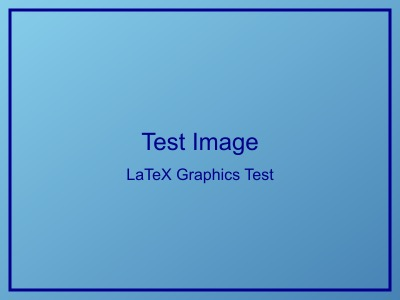
\includegraphics[width=0.8\textwidth]{../../tests/images/test_image.jpg}
    \caption{JPEG 原生支持}
    \label{fig:jpeg_____}
\end{figure}



\subsubsection{2. PNG 格式}

PNG 也是 LaTeX 原生支持的格式,支持透明度。


\begin{figure}[H]
    \centering
    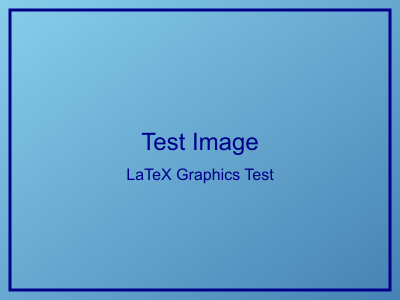
\includegraphics[width=0.8\textwidth]{../../tests/images/test_image.png}
    \caption{PNG 原生支持}
    \label{fig:png_____}
\end{figure}



\subsection{转换后支持的格式}


\subsubsection{3. BMP 转换为 PNG}

BMP 格式通过转换工具转换为 PNG 后支持。


\begin{figure}[H]
    \centering
    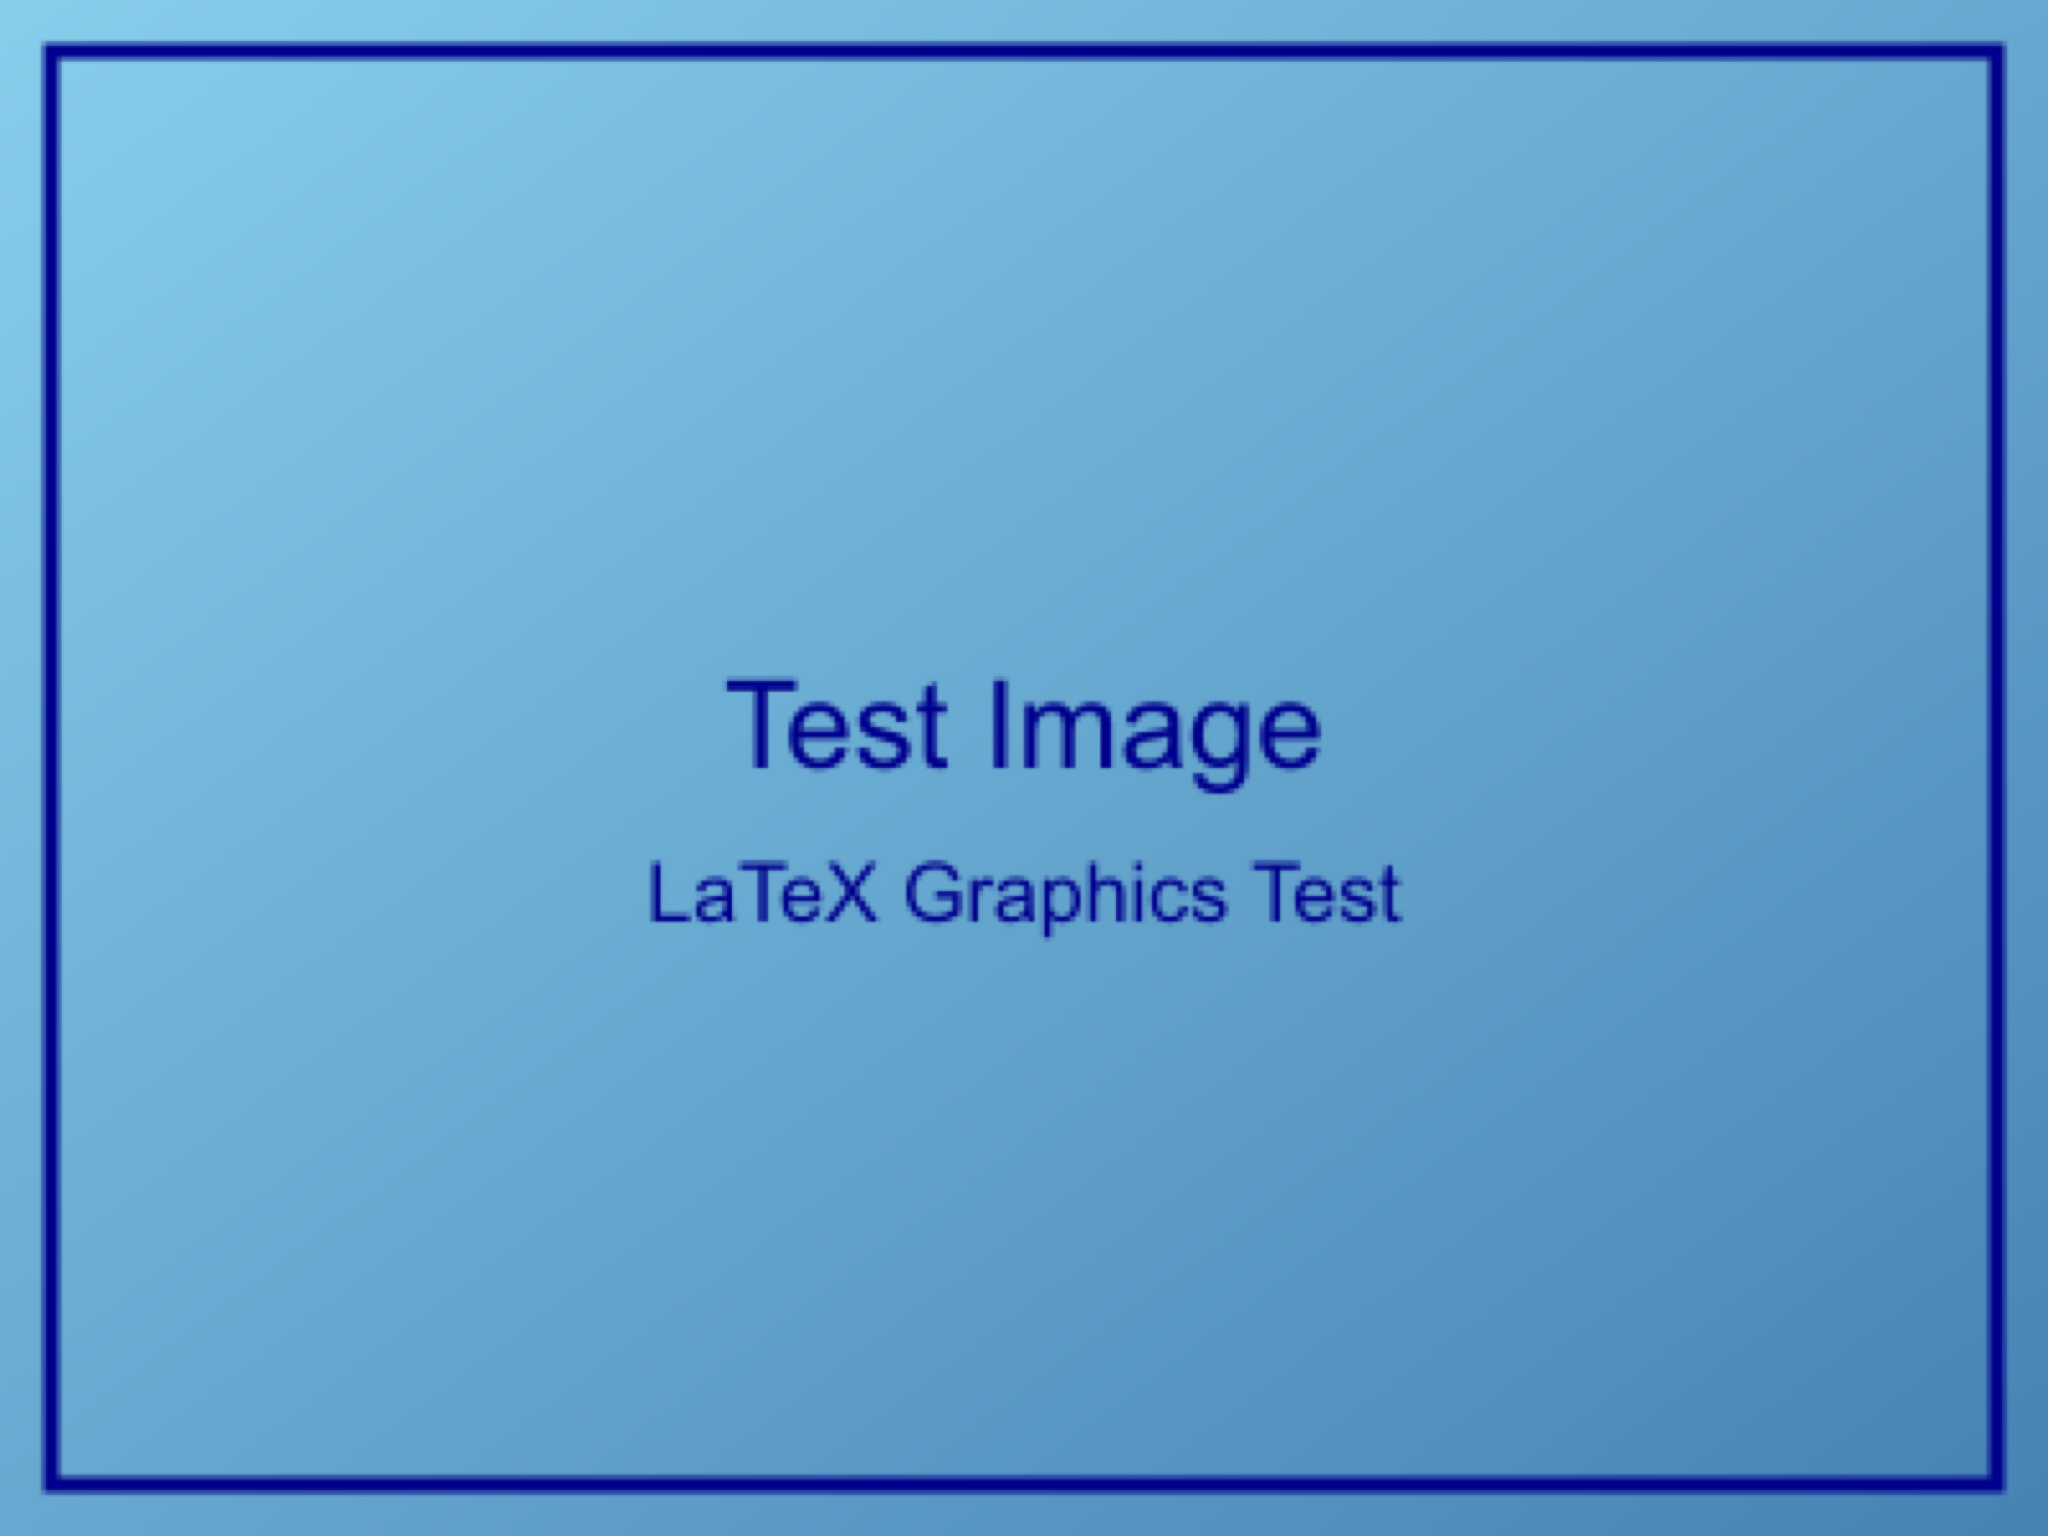
\includegraphics[width=0.8\textwidth]{../../tests/images/converted/test_image.png}
    \caption{BMP 转换支持}
    \label{fig:bmp_____}
\end{figure}



\subsubsection{4. TIFF 转换为 PNG}

TIFF 格式通过转换工具转换为 PNG 后支持。


\begin{figure}[H]
    \centering
    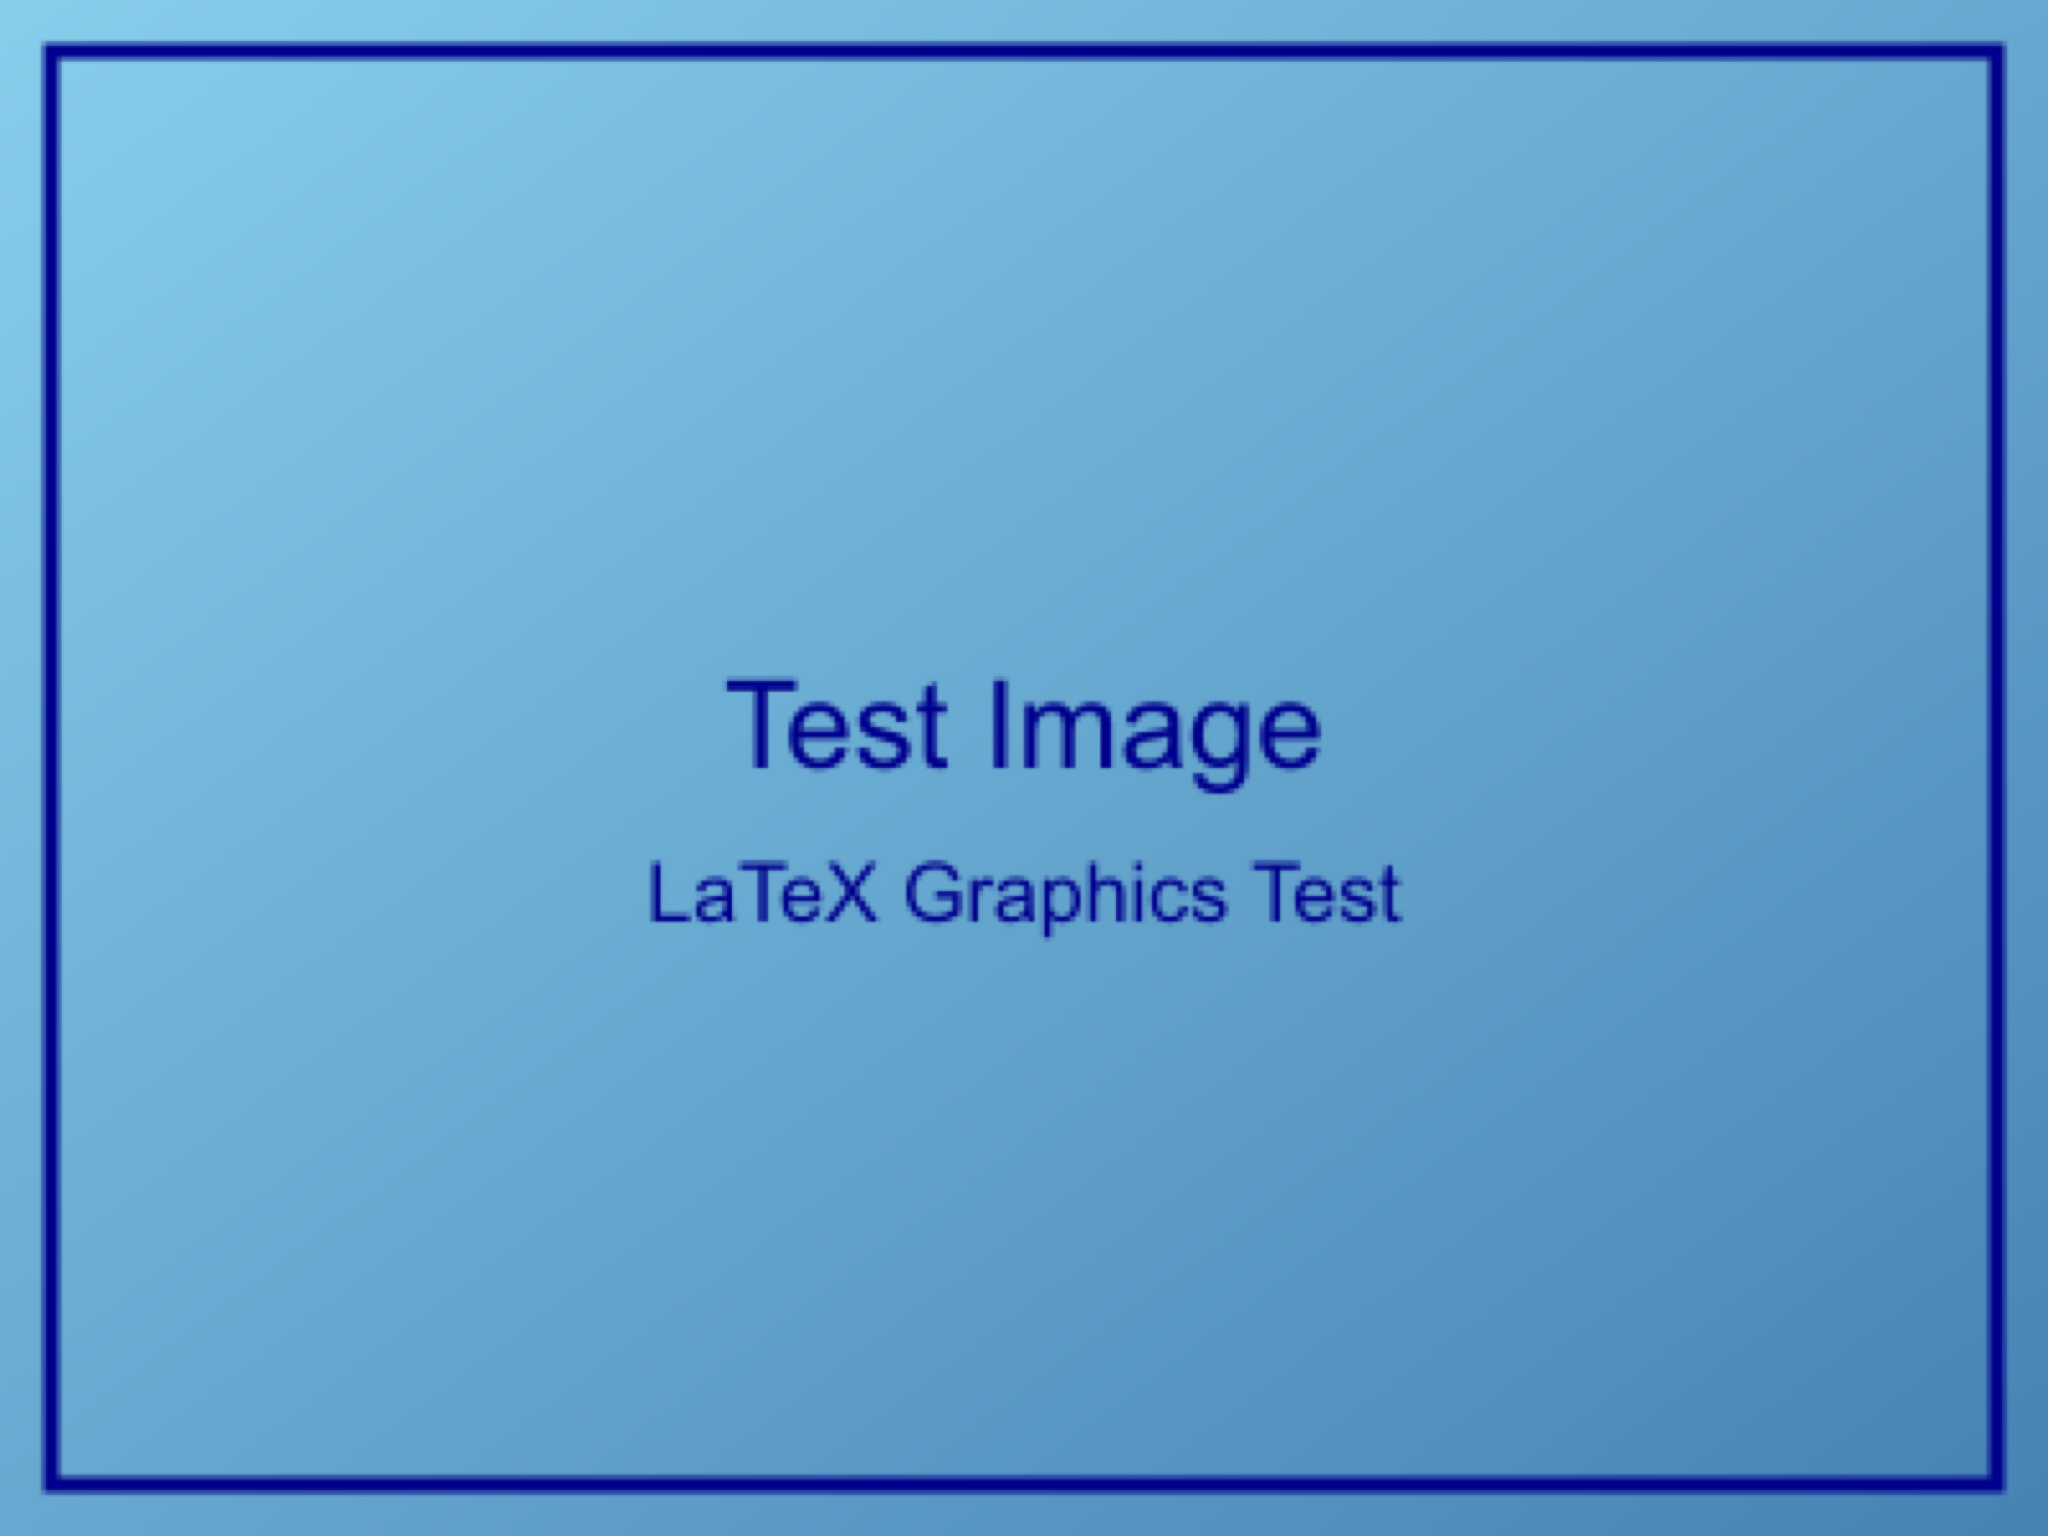
\includegraphics[width=0.8\textwidth]{../../tests/images/converted/test_image.png}
    \caption{TIFF 转换支持}
    \label{fig:tiff_____}
\end{figure}



\subsection{图片处理功能验证}


\subsubsection{路径解析}

\subsubsection{格式兼容性}

\subsubsection{LaTeX 代码生成}

每个图片都生成标准的 figure 环境:


\begin{lstlisting}[language=TeX, basicstyle=\ttfamily\small, breaklines=true]
\begin{figure}[H]
    \centering
    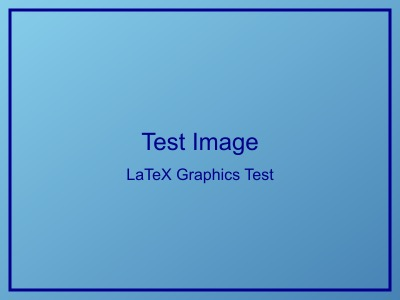
\includegraphics[width=0.8\textwidth]{../../tests/images/test_image.jpg}
    \caption{图片标题}
    \label{fig:图片标签}
\end{figure}

\end{lstlisting}


\subsection{图片转换工具状态}


\subsubsection{可用转换工具}

\subsubsection{支持的输入格式}

BMP, TIFF, TIF, GIF, WebP, SVG, ICO, PSD, RAW


\subsubsection{转换目标格式}

所有不兼容格式都转换为 PNG


\subsection{性能和质量}


\subsubsection{文件大小对比}

\subsubsection{转换质量}

\subsection{测试结果预期}


\subsubsection{PDF 编译}

\subsubsection{文件管理}

\subsection{使用建议}


\subsubsection{最佳实践}

\subsubsection{性能优化}

这个测试验证了 MD2LaTeX 改进版的完整图片处理能力!


\end{document}
